\documentclass[12pt,a4paper]{article}
\usepackage{graphicx}
\usepackage[catalan]{babel}
\usepackage[utf8]{inputenc}
\usepackage[T1]{fontenc}
\usepackage{times}
\usepackage{amsmath}
\usepackage{listings}
\usepackage{amssymb}
%\usepackage{geometry}
\usepackage{url}
\newcounter{exercises}
\setcounter{exercises}{0}
\newtheorem{exer}[exercises]{Pregunta}
\newtheorem{exers}{Exer}

%\geometry{a4paper,tmargin=25mm,bmargin=25mm,lmargin=25mm,rmargin=25mm}

%\pagestyle{empty}

\begin{document}

\section*{Xarxes d’Ordinadors i Internet \\ Curs 2020-2021}
\section*{Pràctica 1: \textit{Simulacions de Xarxa: Protocols de capa física i d'enllaç de dades.}}

\vspace*{0.5cm}
\section{Introducció}


\subsection*{Protocols de xarxa}
L'existència de xarxes de computadors és possible gràcies a la combinació de diversos protocols de comunicació, aquests protocols estableixen un conjunt de conceptes comuns que permeten l'intercanvi de dades entre tota mena de dispositius de xarxa. Aquests protocols s'organitzen en capes i s'agrupen en forma de pila. Les dues classificacions més utilitzades són el model OSI (Open Systems Interconnection) \cite{osi} i el model estàndard que s'utilitza a Internet, la pila de protocols TCP/IP \cite{internet}.

\begin{figure}[!ht]
  \begin{center}
    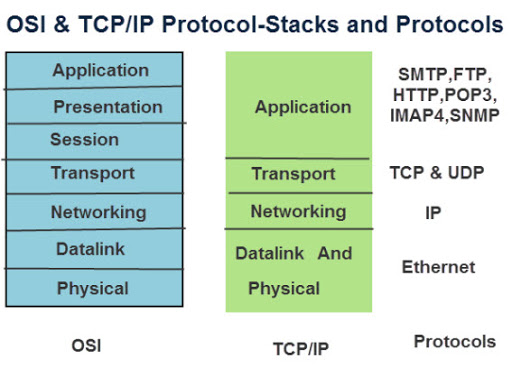
\includegraphics[width=0.7\textwidth]{protocol-stack}
    \caption{Comparativa de les piles - ISO i TCP/IP}
    \label{osi-stack}
  \end{center}
\end{figure}

Les capes inferiors gestionen conceptes del medi físic (freqüències d'ona, modulació, etc.), a mesura que anem pujant de capa els protocols defineixen conceptes més abstractes, com poden ser el format o l'ordre dels missatges. Finalment el nivell més alt (capa d'aplicació) serà en el que se situarien les aplicacions de software que utilitzem comunament (navegadors, client de correu, etc.). Aquest model aporta gran flexibilitat, ja que permet la comunicació de dispositius sempre que comparteixin el mateix protocol a la capa superior, independentment de la tecnologia utilitzada a les capes inferiors.

En aquesta pràctica ens centrarem en les capes físiques i d'enllaç de dades, estudiarem diversos escenaris de xarxa amb dispositius i medis variats, i analitzarem el comportament dels protocols que s'utilitzen en cada cas. Per fer aquesta pràctica utilitzarem dos tipus d'eines, un simulador de xarxa i un analitzador de tràfic

\subsection*{Simuladors de Xarxa}
% TO DO Millorar
Els simuladors de xarxes són programes que modelen el comportament de les xarxes, ja sigui a través de models matemàtics o a través de l'observació directa del tràfic o de les traces generades. Els simuladors permeten predir el funcionament d'una xarxa en funció d'una sèrie d'atributs de l'entorn que es poden modificar. A nivell d'administració de xarxes, l'ús de simuladors és molt útil per estudiar els efectes de les futures ampliacions o modificacions que pugui patir una xarxa.

% En l'àmbit acadèmic, els simuladors també són molt utilitzats per a mesurar i predir el rendiment de nous protocols, sistemes o topologies i comparar-los amb d'altres existents sense necessitat d'implementar físicament tots els canvis. D'aquesta forma, s'aconsegueix un gran estalvi en temps i diners.


%%%%%%%%%%%%%%%%%%%%%
% OPNET
%%%%%%%%%%%%%%%%%%%%%

En aquesta pràctica utilitzarem Network Simulator 3 (NS-3) \cite{ns3}. Aquest és un simulador de xarxa per a entorns Linux que ofereix una API amb la qual es poden crear scripts de simulació en llenguatge C++ o Python. El simulador s'executa com aplicació de consola, però en cas de desitjar-ho tenim la possibilitat de visualitzar els resultats mitjançant una GUI. NS-3 suporta totes les tecnologies de xarxa més habituals (Ethernet, LTE, WiFI, etc\dots) i disposa de models per cada tecnologia. A l'hora de configurar-lo, tots els elements es basen en una llista d'atributs sobre la qual tenim un gran control.

% Riverbed Modeler recull qualsevol tipus d'informació (és molt configurable) sobre les simulacions que executem, a més, realitza gràfics i estadístiques sobre aquesta informació i permet fer comparacions molt fàcilment. Com que utilitzarem una llicència acadèmica, la quantitat de tràfic que podem simular és limitada (no més d'una hora de funcionament).

\subsection*{Analitzadors de paquets}
Un analitzador de paquets és un programa informàtic que captura les trames generades en una xarxa d'ordinadors. A més fa una conversió del tràfic de xarxa en un format entenedor pels humans i mitjançant la seva interficie gràfica  ens permet visualitzar aquesta informació de forma simple.

En aquesta pràctica utilitzarem Wireshark \cite{wireshark}. Wireshark és un programari lliure i de codi obert programat en C++ que inclou les funcionalitats de captura i visualització de paquets. El farem servir principalment per visualitzar el tràfic de xarxa generat a les simulacions de NS-3.

\subsection*{Encapsulat de dades}
\begin{figure}[!ht]
  \begin{center}
    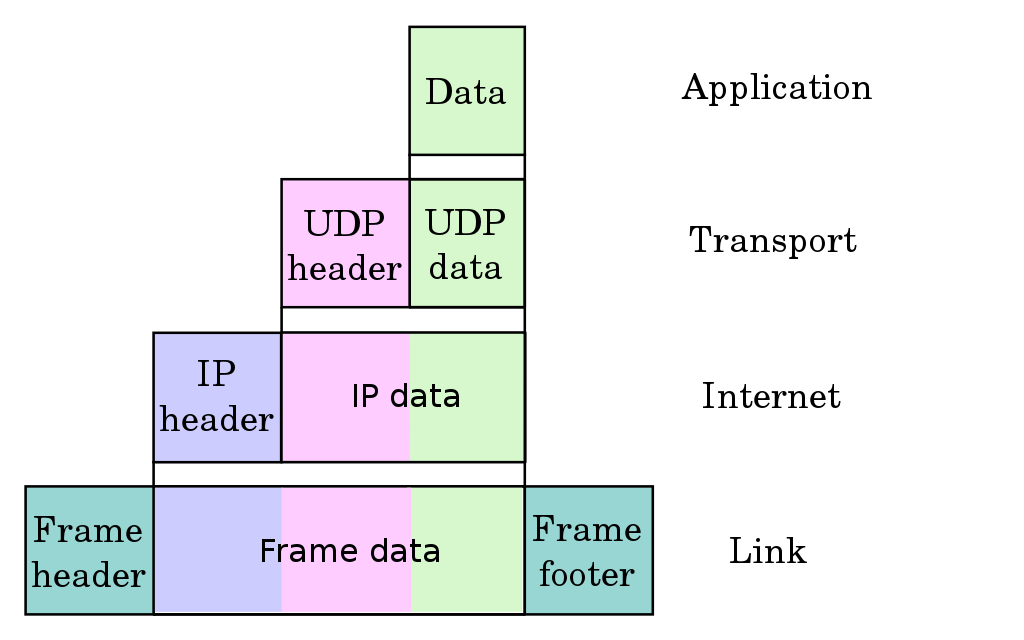
\includegraphics[width=0.7\textwidth]{encapsulation}
    \caption{Encapsulation of application data descending through the layers}
    \label{osi-stack}
  \end{center}
\end{figure}
Foto del wireshark

\section{Guió de la pràctica}

\section*{Observacions}

 \begin{tabular}{||p{12cm}||}
 \hline\hline
 \begin{itemize}
 \item Aquesta pràctica es realitza a dins de la màquina virtual Linux que vau preparar a la Pràctica 0. Podeu iniciar sessió amb les credencials: 
   \newline \texttt{usuari:} \textbf{alumne}
   \newline \texttt{password:} \textbf{alumne}
 \item Per aquesta pràctica necessitareu fer servir la consola de sistema, hi podeu accedir fent clic a \textbf{Home} $\rightarrow$ \textbf{Terminal Emulator} o bé clic dret a l'escriptori i seleccionar \textbf{Open Terminal Here} al menu contextual.
 
 \item El directori d'aquesta pràctica és: \textbf{/home/alumne/labs/lab1/}, es recomana que siteu el vostre terminal en aquest directori (feu servir la comanda \textbf{cd}). A dins trobareu la següent estructura de directoris:
    \begin{itemize}        
        \item\textbf{simulation-scripts}: Trobareu els scripts de simulació a utilitzar durant la pràctica.
        \item\textbf{lliurament}: Carpeta on heu de desar els arxius abans de generar el zip del lliurament.
        \item\textbf{enunciat}: Trobareu una còpia de l'enunciat i materials auxiliars.
    \end{itemize}
 
 \item El contingut de la carpeta \textbf{simulation-scripts} es restaura cada cop que tanqueu sessió, cuaqlsevol modificació als scripts originals es perdrà. Això només s'aplica als arxius originals, per tant, si necesiteu realitzar algun cambi de forma persisten, haureu de desar com un nou arxiu amb nom diferent.
 
 \item Cada execució del simulador donarà com a resultat diversos fitxers amb extensió \textbf{pcap}. Els podeu visualitzar amb \textbf{Wireshark}, simplement heu de fer doble clic a l'arxiu dins de l'explorador de directoris.  
 \end{itemize}
 \\\hline\hline
 \end{tabular}
 \medskip
 
\subsection{Xarxes locals cablejades}

Busqueu informació a Internet i responeu breument a les següents preguntes:

\begin{itemize}
\item \begin{exer}Que és un medi de transmissió? Enumera els 2 tipus de medi més comuns.\end{exer}
\item  \begin{exer} Que és una NIC?\end{exer}
% \item \begin{exer}Que és un cable CAT6? De forma comú amb quin protocol de Capa 2 es fa servir aquest cable?
% Llista 2 tipus de cable d'aquesta mateixa classificació i comenta les diferencies.\end{exer}
% \item Que és un cable creuat? Quina utilitat tenia aquesta tipus de cable?
\item \begin{exer}Que és un Hub? i un Switch? A quina capa del model de xarxa treballa cadascun d'aquests dipositius? Llisteu les principals diferencies.\end{exer}
\item \begin{exer}Que és un domini de colisió? Quants dominis de colisió té una xarxa amb un Hub? I una amb un Switch?\end{exer}
\end{itemize}

A continuació analitzarem de forma pràctica les principals diferencies entre aquests dispositius.

\begin{enumerate}
\item Obriu la carpeta \textbf{simulation-scripts} i localitzeu els arxius: \textbf{hub-scenario.cc} i \textbf{switch-scenario.cc}. Obriu-los amb un editor de text per visualitzar el contingut.

Aquests scripts descriuen una xarxa d'ordinadors fent servir programació orientada a objectes mitjançant l'API que proporciona el simulador ns-3. No és necessari que entengueu tot el que es fa a l'script, però sí que tingueu una idea general, a l'annex \ref{} es desglossa en detall la funcionalitat de cada objecte. 


En aquests scripts es defineix una xarxa local Ethernet amb 4 ordinadors (enumerats de l'1 al 4, on \textbf{n1} seria el \textbf{Node 1}, etc.) enllaçada per cables. En una de les xarxes es fa servir un \textbf{hub} com dispositiu central i a l'altre un \textbf{switch}. En totes dues s'instal·la un stack de protocols TCP/IP a tots els nodes. Addicionalment a dos dels nodes s'instal·la una aplicació que genera tràfic de xarxa de forma intermitent (\textbf{OnOff}): \textbf{n1} envia tràfic a \textbf{n3} i \textbf{n2} envia tràfic a \textbf{n4}. Finalment es defineix que la simulació te una durada de 6 segons.

\item Obriu una consola i executeu la següent comanda:
%\begin{minted}{bash}
\begin{lstlisting}[language=bash]
   ns3 --run "externals/hub-scenario" --vis
\end{lstlisting}
%\end{minted}

Això us obrirà una finestra de visualització on podreu observar la xarxa gràficament. A la part inferior de la finestra podreu veure el panell de control.

  \begin{center}
    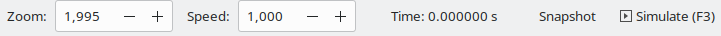
\includegraphics[width=1\textwidth]{simulator}   
    \label{sim-controls}
  \end{center}

\begin{itemize}
 \item Feu clic al botó \textbf{Simulate}.
 \item Executeu la simulació fins a que el comptador \textbf{Time} arribi a 6.0 s
\end{itemize}

Això us permetrà observar la comunicació entre les parelles de nodes.

\item A continuació repetiu la mateixa prova amb l'scenari switch:
%\begin{minted}{bash}
\begin{lstlisting}[language=bash]
   ns3 --run "externals/switch-scenario" --vis
\end{lstlisting}

Fixeu-vos en les diferencies visuals entre els 2 escenaris:
\begin{figure}[!ht]
  \begin{center}
    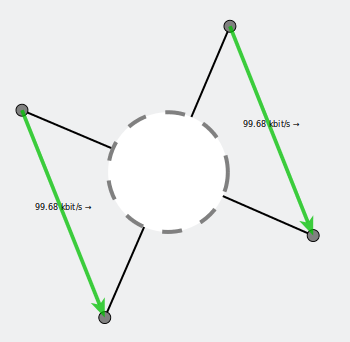
\includegraphics[width=0.4\textwidth]{hub-coms}
    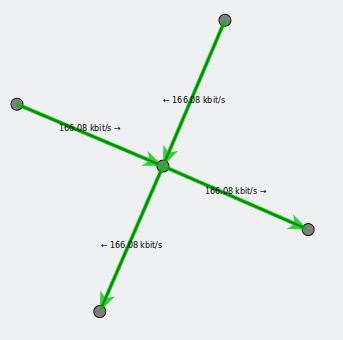
\includegraphics[width=0.4\textwidth]{switch-coms}    
    \label{ns3}
  \end{center}
\end{figure}
\begin{exer} Perquè creieu que els nodes de l'escenari Hub es comuniquen sense que aquest dispositiu aparegui a la simulació? Amb quin dels trets diferenciadors esmentats a la Pregunta 4 associaríeu aquest fet? \end{exer}

\item Si observeu el directori on heu executat les simulacions, veureu que s'han generat multiples fitxers \textbf{.pcap}. Els fitxers segueixen la sintaxi \textbf{<nom-scenari>-<NodeN>-0.pcap}. Cada arxiu conte el trafic rebut per la NIC del node especificat. Per analitzar el continguts del arxius podeu fer servir \textbf{Wireshark}. 

Als arxius de traces apareixerà el trafic generat per tots el protocols de l'stack TCP/IP, per aquest experiment ens interesa veure exclusivament els paquets generats per les aplicacions \textbf{OnOff}. Feu servir la barra de filtre de \textbf{Wireshark} per excloure els continguts no desitjats:
\begin{figure}[!ht]
  \begin{center}
    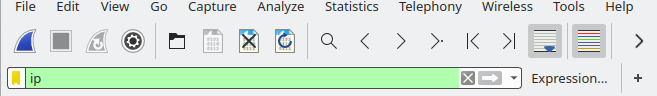
\includegraphics[width=1\textwidth]{wireshark-filter}    
    \label{wireshark}
  \end{center}
\end{figure}

En ambdos escenaris tenim la mateixa situació: n1 envía dades a n3 i n2 envia dades a n4. Tot i això, si observem el traffic de cada node apreciarem diferencies. Compareu els arxius de traffic de cada Node de l'escenari Hub amb el seu homonim de l'escenari Switch.

\begin{exer} Quin trafic podem observar als nodes de l'escenari Hub però no als del Switch? Amb quin dels trets diferenciadors esmentats a la Pregunta 4 associaríeu aquest fet?\end{exer}

Obriu novament al codi font dels scripts de simulació: \textbf{hub-scenario.cc} i \textbf{switch-scenario.cc}. Podreu apreciar que
l'scenari Hub fa servir un canal CSMA compartit entre els 4 nodes. Per altra banda l'escenari Switch fa servir un canal diferent per cada Node connectat al switch.

\begin{exer} A partir d'aquesta observació, amb quin concepte dels definits a les preguntes 1-4 podriem associar el CSMA-channel? \end{exer}

Busqueu informació i contesteu a les següents preguntes:
\begin{exer} Quin és el proposit del protocol CSMA? Perque creieu que és especialment important en una xarxa amb un Hub?\end{exer}
\begin{exer} Com es diu la variant de CSMA que es fa servir en xarxes Ethernet? I la que es fa servir en xarxes WiFi? En que es diferencien? \end{exer}

A continuació observarem el funcionament del protocol CSMA, executeu la següent comanda:

\begin{lstlisting}[language=bash,basicstyle=\footnotesize]
   ns3-run-wparams "externals/hub-scenario" -printChannelState
\end{lstlisting}
Això habilita les traces de log associades al medi físic i al protocol CSMA. Observeu els missatges que han aparegut per consola, les traces segueixen el següent format:
$$
a. Objecte  - b. Event - c. Parameteres - d. Temps $$

\begin{enumerate}
 \item Objecte: Indica quin es l'objecte al que correspon aquest Event, podrá ser un Node  concret o be el canal de comunicació (cable).
 \item Event: Indica quin tipus d'event ha occorregut, els events portaran el suffix \textbf{Phy} si es corresponen a un event de capa física o \textbf{Mac} per capa d'enllaç. Tingueu en compte també les següents abreviatures: Tx = Transmit i Rx = Receive.
 \item Parameters: Informació addicional que pugui ser rellevant per aquest event concret.
 \item Temps: instant de simulació en el que ha occorregut aquest event.
\end{enumerate}

Tenint en compte que \textbf{MacTx} es l'event en el que un frame s'afegeix a la cua de transmissió de la NIC i \textbf{MacPhy} es el moment en que la NIC trasnmet les señals electriques a traves del cable de 
xarxa, Responeu:
\begin{exer} Doneu la llista ordenada de nodes que han enviat informació durant la simulació (si envien informació diversos cops llisteulos multiples vegades).\end{exer}
\begin{exer} Si un node afegeix frames a la seva cua de transmissió abans que un altre, transmetrà \textbf{sempre} les seves dades abans que aquest altre? Doneu un exemple que aparegui a la simulació.
\end{exer}
\begin{exer} Quin es el proposit de l'exponential backoff? Quin impacte creieu que té en l'ordre en que transmeten els nodes? \end{exer}

% \item Podriem crear una xarxa sense fer servir un d'aquest dispositius? En cas afirmatiu, dona 2 exemples de com ho podriem fer (pista: no totes les xarxes fan servir cables).
\end{enumerate}


\subsection{Xarxes locals sense fils}
- Comparar visualment.
- Mirar wireshark protocol d'afegir nodes.


\section{Calendari i fites importants}
% ------------------------------------------------------------------------------------------
%       Calendari i Fites importants 
% ------------------------------------------------------------------------------------------

A continuació es descriu el calendari de les fites relatives a la pràctica:

\begin{itemize}
        \item \textbf{Sessió pràctica}: 24/02/20 i 02/03/20.
	\item \textbf{Lliurament}: 08/03/20.
\end{itemize}

\section{Condicions de lliurament}
% ------------------------------------------------------------------------------------------
%       Condicions de lliurament
% ------------------------------------------------------------------------------------------

\begin{itemize}
  \item L'entrega de la pràctica es farà a través del campus virtual.
  \item Cada grup ha d'entregar un informe en format pdf que contingui les respostes a totes les preguntes d'aquest enunciat.
   \item No s'acceptarà cap informe lliurat fora de plaç.
\end{itemize}

\bibliographystyle{plain}
\bibliography{Prac1}


\end{document}
